\section{L'ultimo degli hacker}

Analizziamo la fase di decadenza degli hacker, qui entra in gioco Richard Stallman.

\subsection{Bibliografia}

\begin{itemize}

\item Steven Levy: \textit{Heroes of the computer revolution};
\item Sam Williams: \textit{Free as in Freedom (2.0): Richard Stallman and the free software revolution}

\end{itemize}

\subsection{Prime esperienze}

Richard Stallman nasce a New York nel 1953 dove si forma dal punto di vista informatico, diventa un esperto di \glossario{Assembler}, di sistemi operativi e di editor di testo. Inizia con le prime esperienze nel centro scientifico di Manhattan, poi lo assumono e inizia a sviluppare programmi in Fortran per il calcolo numerico. Nel 1971 entra ad Harvard e si laurea in Fisica. Scopre in segreto un'affinità con la cultura hacker sviluppatasi al MIT. Venne notato da Russ Noftsker e in seguito assunto al MIT come programmatore di sistemi. Viene preso sotto l'ala protettiva di Richard Greenblatt e Bill Gosper, che gli fanno da mentore.

\begin{figure}[htbp]
\centering
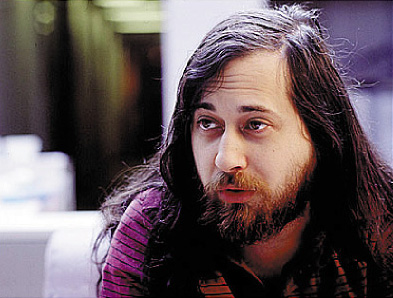
\includegraphics[width=50mm]{images/stallman.jpg}
\caption{Richard Stallmann da giovane}
\end{figure}

\subsection{Emacs}

Una delle prime cose che Stallman fece fu la creazione di \glossario{Emacs}. Inizialmente esso era pensato come un insieme di macro per \glossario{TECO}, utlilizzato da tutti, che era una sorta di linguaggio per scrivere e non era assolutamente real-time. Creò dunque una sorta di editor dentro TECO. Guy Steele ebbe in seguito l'idea di fare un po' di ordine tra le macro (che erano diventate tantissime). Quest'opera fu continuata da Stallman, in modo da avere un insieme più omogeneo. Questo disordine non sarebbe dovuto replicarsi in futuro, bisognava evitare che ciascuno costruisse il proprio insieme di macro. Stallman voleva fare qualcosa di ``sociale'', voleva andare un po' oltre e impedire ulteriori disordini. Quindi si imposero delle restrizioni sulle modifiche delle macro. Questa condizione creò una sorta di comunità in cui i programmatori condividevano gli sforzi di programmazione ed evitavano la dispersione del lavoro. Questo fu il primo gruppo concreto di condivisione del software e il primo mattone della nascita della GPL. Emacs è nato in questo modo, ma poi è stato ritradotto varie volte.

\begin{figure}[htbp]
\centering

\includegraphics[width=20mm]{images/emacs.png}
\caption{Il logo di emacs}
\end{figure}

\subsection{Le prime incursioni}

Allo stesso tempo si iniziarono a vedere le prime debolezze. Il dipartimento di difesa obbligò gli hackers a programmare sui sistemi del dipartimento di \textit{computer science} del MIT, in cui c'era mancanza di accesso libero all'informazione. Arrivarono al punto di fare una sorta di ``sciopero'' nei confronto del laboratorio e bloccarono l'accesso alle succesive versioni di Emacs. Si creò dunque una frattura tra Richard Stallman e la comunità.

Gli hackers cominciarono a migrare e andarono a lavorare altrove per altre società. Comparirono i primi programmi coperti da copyright nel campo dell'\textbf{intelligenza artificiale}.

\subsection{La lisp machine e il collasso}

Richard Greenblatt, un programmatore del MIT, era un'autorità nel settore. Aveva iniziato a giocare con le \glossario{lisp machine} (lisp era un linguaggio ad alto livello) e aveva avuto l'idea di creare una macchina che eseguisse lisp in modo più efficiente e sicuro. Creò una sorta di controllo all'interno di lisp per la gestione delle risorse, aveva modificato la struttura dell'hardware in modo che lisp venisse utilizzato più velocemente. Questo fu un grosso passo avanti, perchè programmare in lisp era molto più comodo che programmare in assembler. Alla lunga riuscì ad ottenere lo stanziamento di fondi per 6 macchine. Si arrivò a produrne 32. Anche per gli hacker era un mondo nuovo, perchè cambiava la visione classica (un solo computer disponibile), ora ogni persona aveva la propria macchina. Pensò dunque di collegare queste 32 macchine per favorire la condivisione. Il progetto è cresciuto a un punto tale che si trasformò in un azienda per la produzione di lisp machine, che in un certo senso era un'estensione del MIT. La visione di Greenblatt era quella di un'azienda \textit{``hacker friendly''}. Russel Noftsker non condivideva molto l'idea, era parte del progetto, ma la sua visione era incompatibile con quella di Greenblatt, pensava che l'azienda non sarebbe stata in grado di produrre grosse modifiche a livello globale.
Nel 1979 si arriva al punto in cui il conflitto esplode (Greenblatt aveva dalla sua un caratteraccio, non teneva conto delle persone). Da un lato non si poteva ``far fuori Greenblatt'', ma dall'altro non c'erano molte persone che volessero continuare con la sua visione (Greenblatt voleva avere l'ultima parola), quindi in sostanza non esisteva un team. Perciò gli diedero un anno di tempo per fondare l'azienda, altrimenti gli altri avrebbero fondato la loro. Riuscì sorprendentemente a creare un'azienda che funzionasse, la \glossario{LMI}, ma dopo un anno gli altri suoi colleghi crearono \glossario{Symbolics}.

\begin{figure}[htbp]
\centering
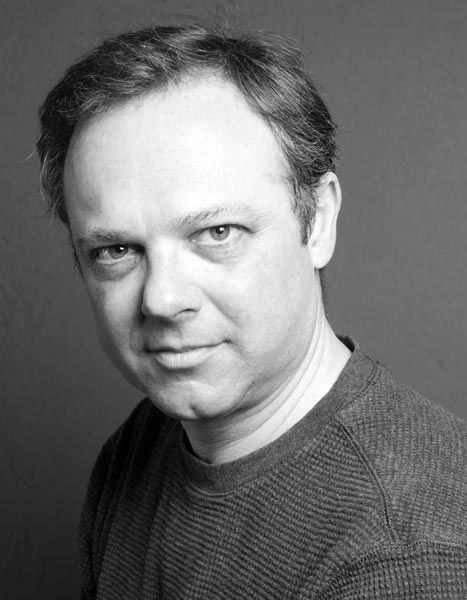
\includegraphics[width=50mm]{images/greenblatt.jpg}
\caption{Richard Greenblatt da giovane}
\end{figure}

\subsection{Lo svuotamento del MIT}

LMI e Symbolics attingono pesantemente dal MIT (concorrenza). Nel 1982 Symbolics rende le proprie modifiche al sistema operativo delle lisp machines proprietario. A questo punto c'è un crollo della comunità, era già molto debole, erano rimasti pochi hackers ma c'era comunque un sistema complesso che andava mantenuto. 
Quindi a un certo punto PDP divenne obsoleto e la comunità si ritrovò di fronte a un problema, bisognava creare una nuova macchina, era necessario prendere tutto il software delle macchine correnti e riscriverlo, e gli hackers non erano abbastanza numerosi. Alla fine si decise di comprare il sistema operativo proprietario di \glossario{Digital} e a partire da esso si creò \glossario{Twenex}, con caratteristiche molto diverse da un sistema standard (sicurezza costruita nel sistema). 
Il gruppo wheel era un gruppo i cui programmatori erano gli unici che potevano divenire amministratori e apportare modifiche alla macchina. In seguito ci fu la nascita di GNU.

\subsection{L'appello}

nel 1983 Richard Stallman fece un appello su \texttt{net.unix-wizards}:

\begin{center}

\textit{``Starting this Thanksgiving I am going to write a complete Unix-compatible software system called GNU (for Gnu’s Not Unix), and give it away free to everyone who can use it. Contributions of time, money, programs and equipment are greatly needed''}.

\end{center}

Le ragioni della scelta di unix furono:

\begin{itemize}

\item Il monopolio della AT\&T;
\item La familiarità con il codice sorgente (e grosso utilizzo da parte delle università), c'era un grande numero di utilizzatori e di sviluppatori;
\item La portabilità (sviluppato in C e non in assembler), sistema che si adattasse alle macchine, su architetture molto diverse.

\end{itemize}

\subsection{GNU Emacs}

La prima cosa che serviva era un programma per eseguire il codice, quindi ci fu un grosso lavoro sul compilatore. Stallman parte dal codice di Gosling e scrive GNU Emacs. L'Emacs del MIT non andava bene, serviva una nuova versione che andasse bene per le macchine piccole. Si erano nel frattempo creati tutta una serie di \textit{cloni} di Emacs, una di quelle era scritta da James Gosling e quest'ultimo concedette a Stallman il codice senza problemi, dal quale potè creare una nuova versione.
Unipress a quel punto minacciò legalmente Emacs (aveva acquistato la versione di Gosling), ma per fortuna di Stallman la versione era stata riscritta praticamente da zero, per cui non ebbe problemi e nel 1985 rilasciò ufficialmente il programma. 
\linebreak
\linebreak
Stallman decise di pensare bene a una licenza per la versione, basandosi su GNU. La licenza era basata principalmente sulla licenza implicita della comunità Emacs. È il primo grosso progetto di GNU, che sotto sotto era una GPL. A partire da esso si svilupparono tutta un'altra serie di progetti, bisognava creare dunque una licenza che fosse comune a tutti. Gilmore suggerì dunque il cambio di nome e nacque la GNU general public license che venne distribuita in versione 1.0 con il rilascio di \glossario{gdb}.

\subsection{L'incontro con BSD}

AT\&T cominciò a focalizzarsi sull'utilizzo di Unix a scopo commerciale e nel frattempo si sviluppò BDS, una distribuzione di Unix derivata con scopi accademici e con diversi contributi esterni. L'idea era di trasformare i loro sistemi operativi \textit{batch} con una versione di Unix.
Due studenti si erano appassionati e avevano reso una versione migliore di BSD, aggiungendo tutta una serie di cose, iniziando dapprima a effettuare modifiche esterne e poi interne. Quindi si formò una distribuzione indipendente, ma c'era la necessità della licenza AT\&T. Stallman convinse Bostic e i suoi a creare una versione completamente libera (all'inizio era un po' deficitaria ma col tempo si è messa in pari). A questo punto c'era un sistema operativo (e un kernel) libero.

\subsection{Anni 80-90}

Intorno alla costellazione GNU ci furono vari programmatori che iniziarono a rilasciare codice sotto licenza GPL. Bruce Perens rilascia \textit{electric fence} sotto licenza GPL, una libreria per le chiamate all'allocazione di memoria. Bruce Perens sarebbe diventato in seguito il project leader di Debian.
\linebreak
\linebreak
GPL stava dunque divenendo una licenza molto importante. Rich Marin fonda \glossario{Prime Time Freeware}, un'azienda che rilascia software solo sotto GPL. L'azienda \glossario{Cygnus} con Micheal Tiemann aveva cominciato a lavorare al progetto \glossario{gcc}, aggiungendo il supporto al C++. Il progetto era quella di contribuire (fare modifiche) al gcc e poi rivenderlo. L'idea ebbe un notevole successo. Cygnus venne fondata nel 1990 e per la fine dell'anno valeva 725000\$ in supporto e contratti.

\subsection{Espansione del progetto GNU}

Il progetto GNU si espanse in modo molto rapido e virale. Di seguito vengono riportati i maggiori rilasci dei primi anni:

\begin{itemize}

\item gcc;
\item Libc (1987);
\item Bash (la shell), fileutils (gestione dei file), sh-utils, textutils (gestione dei testi);
\item Ghostscript;
\item Textinfo (formattazione della documentazione, l'html lo renderà obsoleto);
\item Yakk, make, ...

\end{itemize}